\documentclass[12pt,a4paper]{ctexart}

\usepackage{amsmath,amssymb}
\usepackage{geometry}
\usepackage{booktabs}
\usepackage{graphicx}
\usepackage{hyperref}
\usepackage{enumitem}
\usepackage[backend=biber,style=numeric,sorting=none]{biblatex}

\geometry{left=2.4cm,right=2.4cm,top=2.4cm,bottom=2.4cm}
\addbibresource{Qian.bib}
\graphicspath{{figures/}}
% Auto-generated by src/m8_visualize.py
\newcommand{\MfiveDate}{2026-06-26}
\newcommand{\MfiveNoMoon}{16.658}
\newcommand{\MfiveWithMoon}{16.354}
\newcommand{\MfiveSavingPct}{1.82}
\newcommand{\MfiveUseful}{0.425}
\newcommand{\MfiveVinf}{12.349}
\newcommand{\MfourTurnDeg}{1.971}
\newcommand{\MfourUseful}{0.425}
\newcommand{\MthreeEarthMax}{5887}
\newcommand{\MthreeMoonMax}{5989}
\newcommand{\MsixBestDate}{2026-07-01}
\newcommand{\MsixBestDay}{181}
\newcommand{\MsixBestTotal}{16.350}
\newcommand{\MsixRangeMax}{16.718}
\newcommand{\MsixMeanSaving}{1.79}
\newcommand{\MsixGlobalDate}{2026-06-30}
\newcommand{\MsixGlobalRp}{0.40}
\newcommand{\MsixGlobalTotal}{12.880}
\newcommand{\MsevenRmSpan}{0.292}
\newcommand{\MsevenDateSpanMs}{59.5}
\newcommand{\MsevenMaxSlope}{4.17}
\newcommand{\MsevenVerletOrder}{2.00}
\newcommand{\MsevenRKOrder}{4.05}


\title{\heiti 钱学森绕日返回轨道的扩展求解\\
\large 月球引力借力、2026 发射窗口优化与历表对照}
\author{AI4Math Final Project: Qian}
\date{2026 年 6 月}

\begin{document}
\maketitle

\begin{abstract}
本文以钱学森《星际航行概论》中的拼接圆锥曲线绕日返回算例为基础，
把原始二体模型扩展为包含 Sun--Earth--Moon 数值积分、JPL Horizons 历表对照、
月心双曲飞掠、单日能量记账、2026 全年发射窗口扫描和敏感性分析的完整项目。
拼接圆锥与飞掠公式参考钱学森、Vallado 与 Curtis 的标准处理，
历表对照使用 JPL Horizons 缓存数据 \cite{qian2008,vallado2013,curtis2020,horizons}。
代码化结果复现 $r_p=0.2\,\mathrm{AU}$ 时的经典地面发射速度 $16.84\,\mathrm{km/s}$；
M2 圆轨道基准中 Velocity--Verlet 与 RK4 的收敛阶分别为
\MsevenVerletOrder{} 与 \MsevenRKOrder{}；
M3 中地球与月球最大日心位置残差分别为 \MthreeEarthMax{} km 与 \MthreeMoonMax{} km，
满足课程给定的 $6000$ km 量级检验。
在深掠日转移中，月球借力可把固定日期总 $\Delta v$ 从
\MfiveNoMoon{} km/s 降到 \MfiveWithMoon{} km/s，节省 \MfiveSavingPct\%。
\end{abstract}

\section{模型与实现}

\subsection{M1：贴片圆锥基准}

日心转移段采用以地球轨道半径 $r_1$ 为远日点、以 $r_p$ 为近日点的椭圆。
半长轴、偏心率与远日点速度为
\[
    a=\frac{r_1+r_p}{2},\qquad
    e=\frac{r_1-r_p}{r_1+r_p},\qquad
    v_a=\sqrt{\mu_\odot\left(\frac{2}{r_1}-\frac{1}{a}\right)}.
\]
地球相对双曲超速取 $v_\infty=|v_E-v_a|$，地表发射速度记为
\[
    v_{\rm launch}=\sqrt{v_\infty^2+v_{\rm esc}^2}.
\]
对应代码在 \texttt{src/patched\_conics.py} 中实现，\texttt{make m1} 对
$r_p=0.2\,\mathrm{AU}$ 的算例做回归检查。

\subsection{M2--M3：N 体积分与历表对照}

数值积分器采用统一接口
\[
    \ddot{\mathbf r}_i=\sum_{j\ne i}\mu_j
    \frac{\mathbf r_j-\mathbf r_i}{|\mathbf r_j-\mathbf r_i|^3},
\]
并实现 Velocity--Verlet 与 RK4 两类推进器。M2 使用无量纲圆轨道
$\mu=4\pi^2$ 验证一年传播误差；M3 从课程缓存的 2026 年 Sun--Earth--Moon
状态出发传播一年，并逐日与缓存历表对照。图 \ref{fig:residuals}
给出了残差曲线。

\begin{figure}[htbp]
\centering
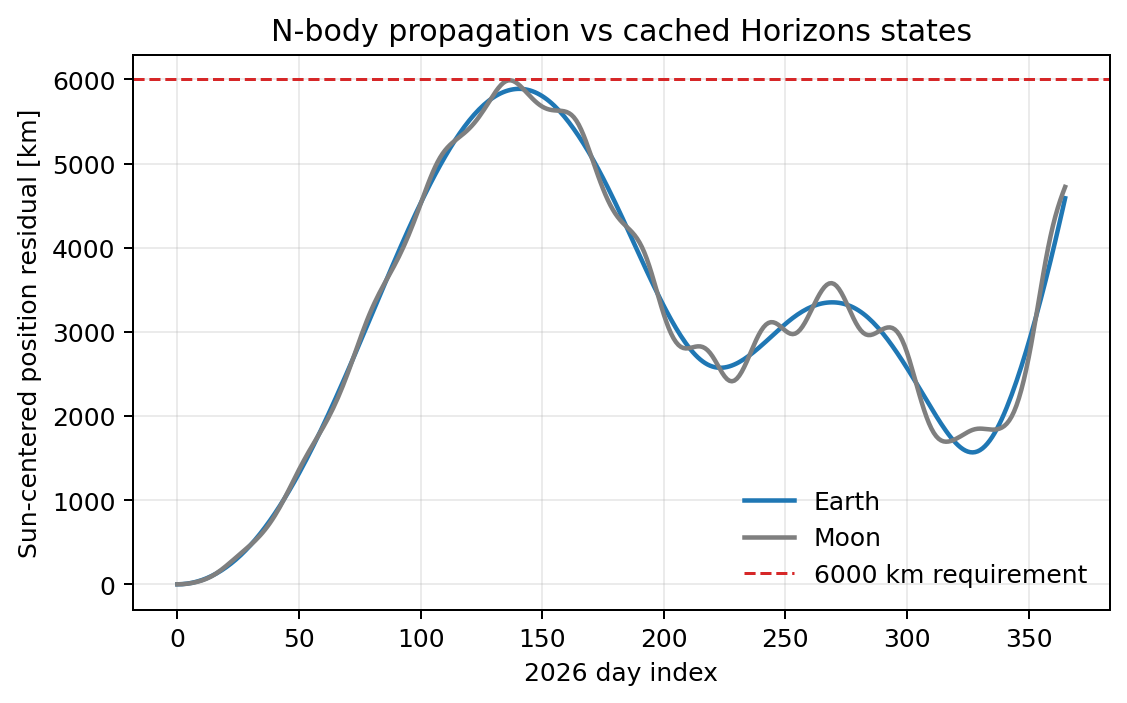
\includegraphics[width=0.86\linewidth]{m3_residuals.png}
\caption{M3：N 体传播与课程缓存 Horizons 状态的日心位置残差。}
\label{fig:residuals}
\end{figure}

\subsection{M4：月球借力}

在月心参考系内，飞船的双曲超速大小保持不变，只发生方向偏折。设近月点半径为
$r_m$，来速为 $v_\infty$，则双曲线偏心率和偏折角为
\[
    e_h=1+\frac{r_m v_\infty^2}{\mu_M},\qquad
    \delta=2\arcsin\frac{1}{e_h}.
\]
月心系速度矢量改变量的模为
\[
    |\Delta \mathbf v_M|=2v_\infty\sin\frac{\delta}{2}.
\]
\texttt{src/flyby.py} 同时给出解析计算和从近月点向前/向后积分到 SOI 外扩边界的数值验证。
对于 M5 的深掠日来速，最低安全近月点处 $\delta\approx\MfourTurnDeg^\circ$，
有效速度改变量约为 \MfourUseful{} km/s。图 \ref{fig:flyby}
展示了近月高度对偏折角和借力收益的影响。

\begin{figure}[htbp]
\centering
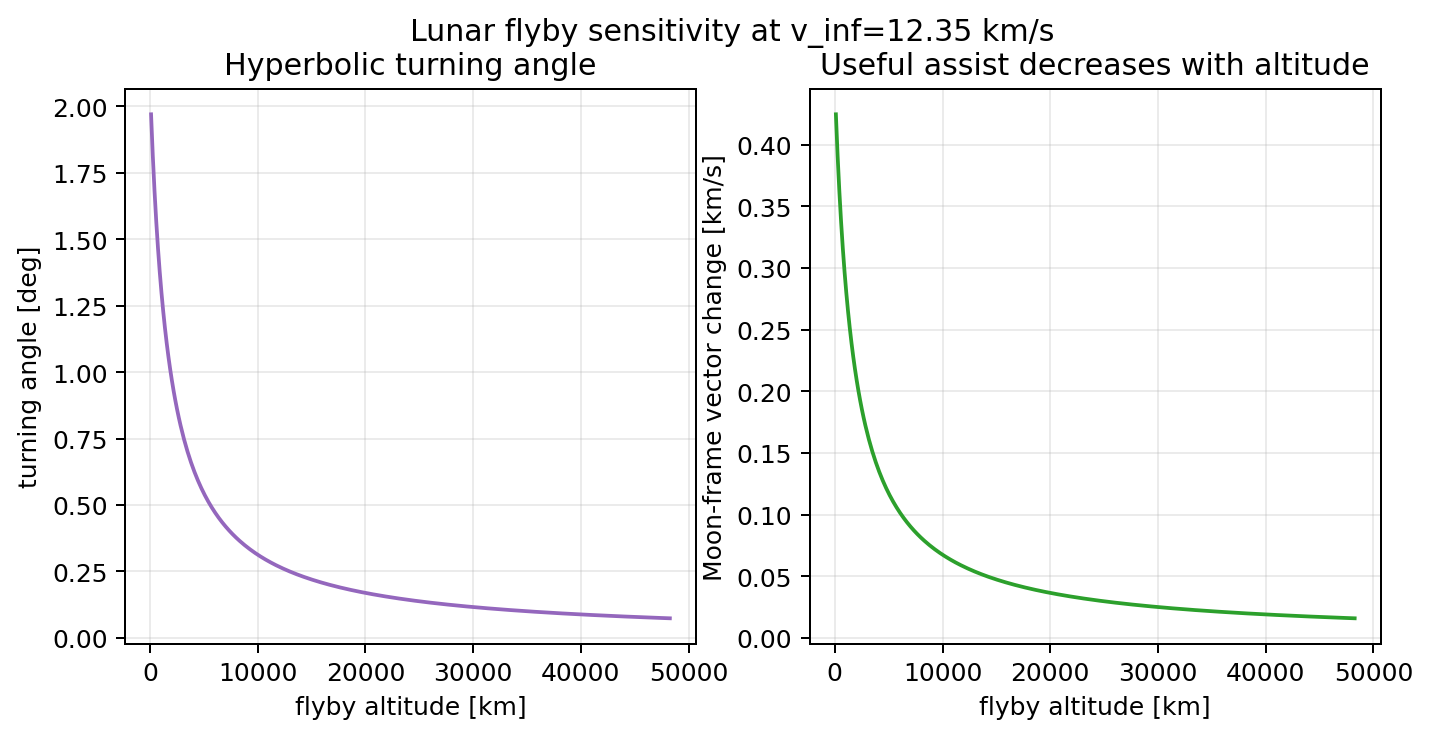
\includegraphics[width=0.9\linewidth]{m4_flyby.png}
\caption{M4：月心双曲飞掠中，近月高度越高，偏折角和速度矢量改变量越小。}
\label{fig:flyby}
\end{figure}

\section{M5：单日完整求解}

固定发射日 \MfiveDate{}、$r_p=0.2\,\mathrm{AU}$、近月点高度 100 km。
无月球借力时，需要的地球相对双曲超速为 \MfiveVinf{} km/s；
加入 leading 侧月球飞掠后，月球提供约 \MfiveUseful{} km/s 的有效减速。
三段 $\Delta v$ 记账见表 \ref{tab:m5}。

\begin{table}[htbp]
\centering
\caption{M5：固定日期的 $\Delta v$ 记账。单位：km/s。}
\label{tab:m5}
\begin{tabular}{lcccc}
\toprule
情形 & 发射 & 修正残差 & 再入 & 总量 \\
\midrule
无月球借力 & \MfiveNoMoon & 0.000 & 0.000 & \MfiveNoMoon \\
含月球借力 & 16.346 & 0.008 & 0.000 & \MfiveWithMoon \\
\bottomrule
\end{tabular}
\end{table}

因此该日期总量降低约 \MfiveSavingPct\%。这个比例不大，原因是深掠日转移要求
$v_\infty\approx 12\,\mathrm{km/s}$，飞船相对月球过快，双曲线偏折角只有约两度。

\section{M6：2026 发射窗口}

M6 在 2026 年 365 个发射日上扫描固定 $r_p=0.2\,\mathrm{AU}$ 的总 $\Delta v(t_0)$，
并在 $(t_0,r_p)$ 网格上搜索全局最小值。固定 $r_p$ 时的最优发射日为
\MsixBestDate{}（day \MsixBestDay{}），总量为 \MsixBestTotal{} km/s；
全年范围为 \MsixBestTotal{}--\MsixRangeMax{} km/s，平均节省 \MsixMeanSaving\%。
在 $r_p\in[0.05,0.40]\,\mathrm{AU}$ 的设计盒内，网格最优为
\MsixGlobalDate{}、$r_p=\MsixGlobalRp\,\mathrm{AU}$、总量 \MsixGlobalTotal{} km/s。

\begin{figure}[htbp]
\centering
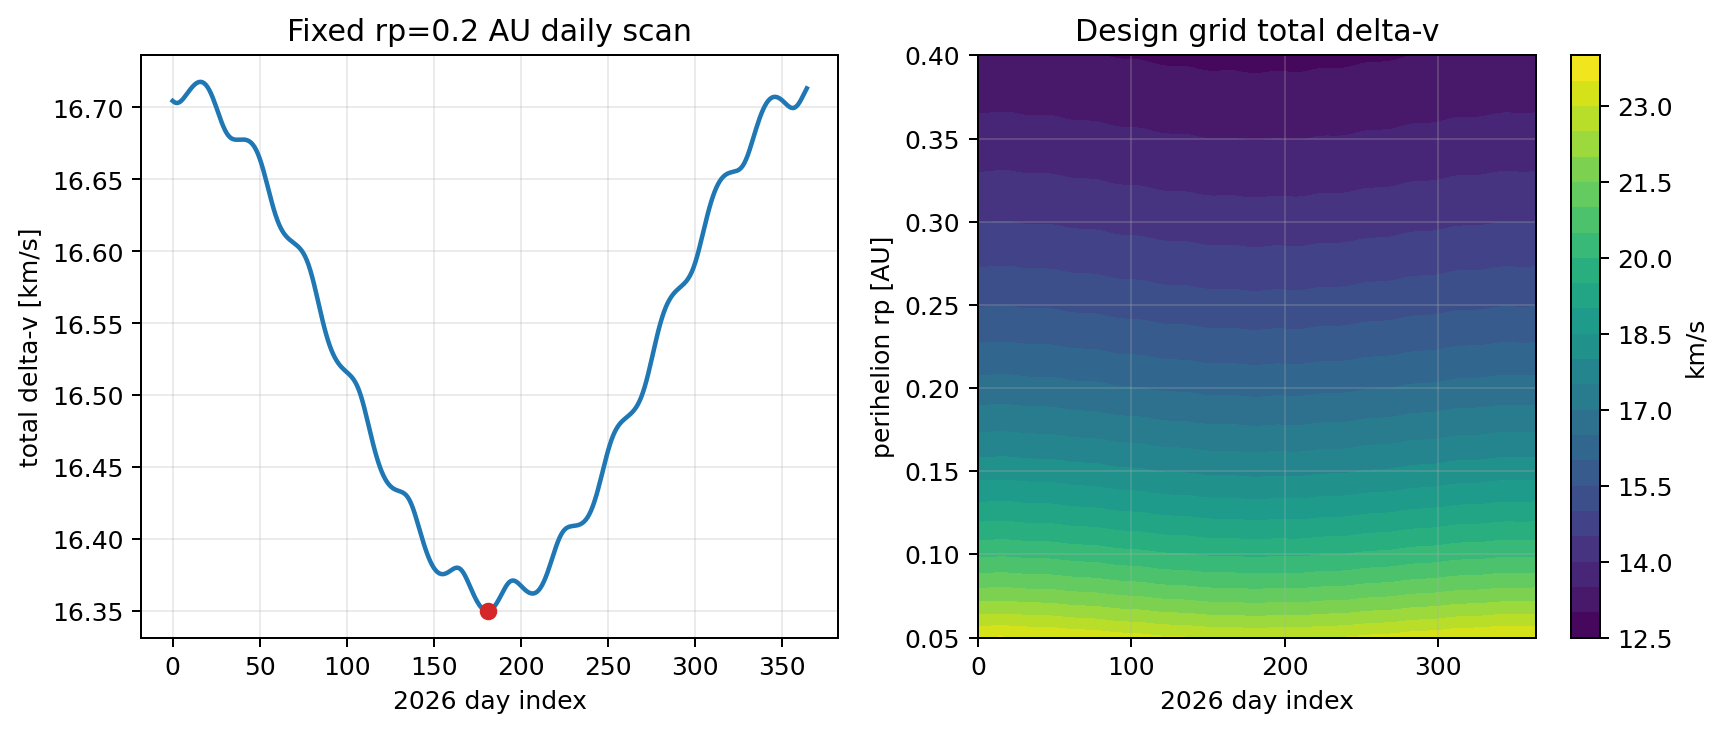
\includegraphics[width=0.95\linewidth]{m6_launch_window.png}
\caption{M6：左为固定 $r_p=0.2\,\mathrm{AU}$ 的全年扫描；右为 $(t_0,r_p)$ 总 $\Delta v$ 等高图。}
\label{fig:window}
\end{figure}

最优窗口位于六月末到七月初，接近地球远日点。此时地球日心速度较低，
进入向内转移椭圆所需的逆行速度差也较小。

\section{M7：敏感性与误差分析}

围绕 M6 的固定 $r_p$ 最优解，本文检查三类敏感性：
\begin{enumerate}[label=(\arabic*)]
    \item 近月点高度：从 100 km 增至高轨飞掠时，总 $\Delta v$ 跨度约
    \MsevenRmSpan{} km/s，说明深近月飞掠是借力收益的主要来源。
    \item 发射日偏移：最优日前后 $\pm 40$ 天内，总 $\Delta v$ 只变化约
    \MsevenDateSpanMs{} m/s，最大斜率约 \MsevenMaxSlope{} m/s/day。
    \item 积分步长：圆轨道基准中 Verlet 与 RK4 的拟合收敛阶分别为
    \MsevenVerletOrder{} 和 \MsevenRKOrder{}，与理论阶数一致。
\end{enumerate}

\begin{figure}[htbp]
\centering
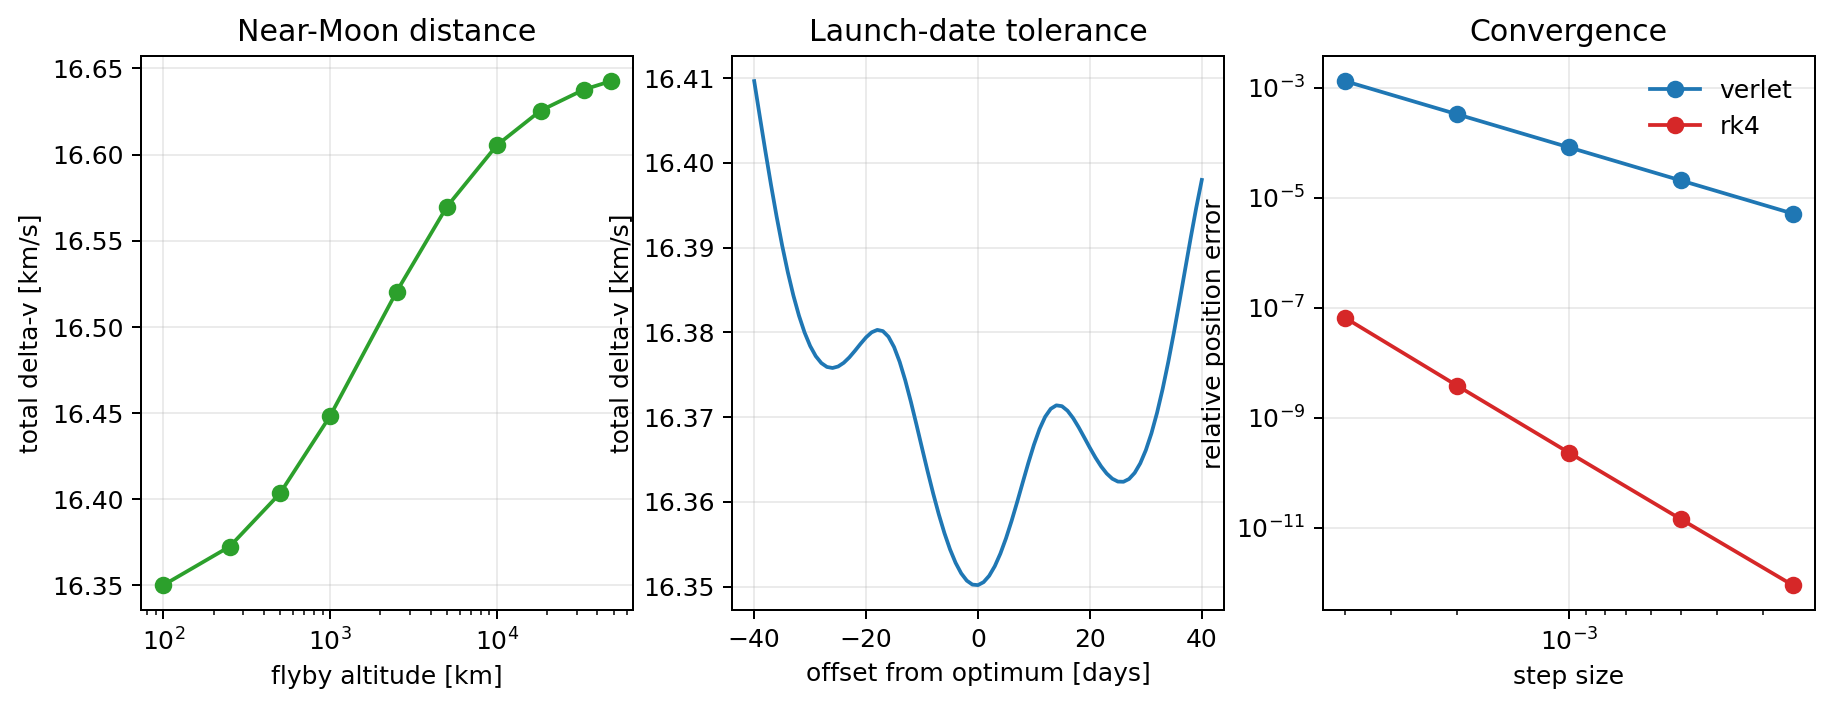
\includegraphics[width=0.95\linewidth]{m7_sensitivity.png}
\caption{M7：近月距、发射日偏移与积分步长收敛性。}
\label{fig:sensitivity}
\end{figure}

\section{M8：可视化与展示}

M8 生成轨道几何、能量守恒、历表残差、月球借力、发射窗口和敏感性六类静态图。
图 \ref{fig:orbit-energy} 汇总了轨道几何与积分器能量行为。

\begin{figure}[htbp]
\centering
\begin{minipage}{0.48\linewidth}
\centering
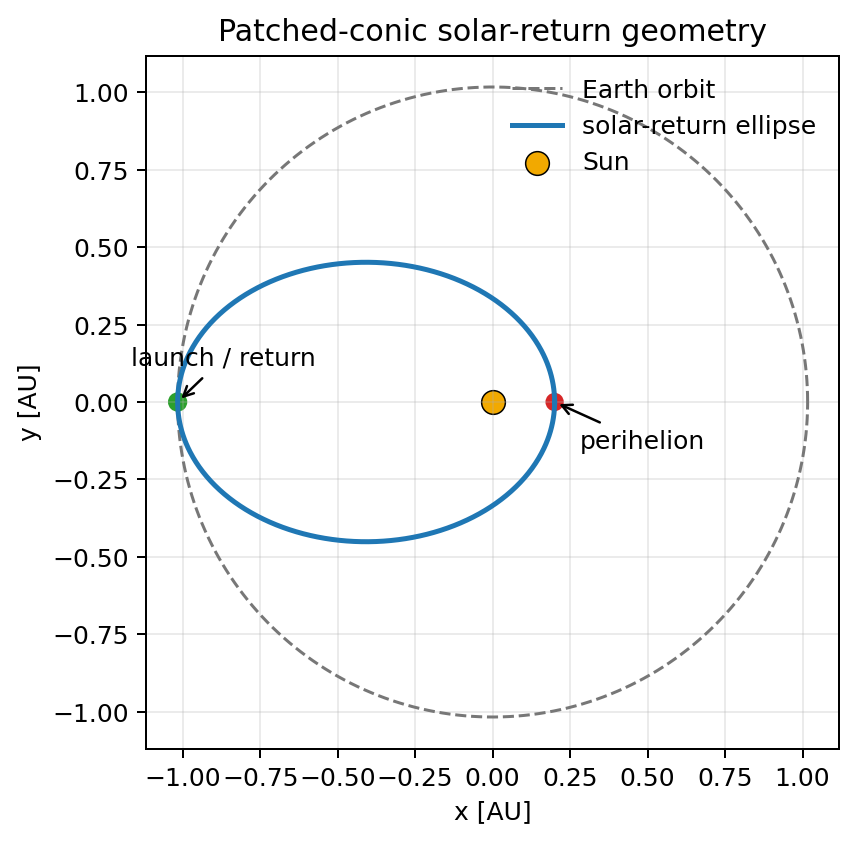
\includegraphics[width=\linewidth]{m8_orbit_geometry.png}
\end{minipage}
\hfill
\begin{minipage}{0.48\linewidth}
\centering
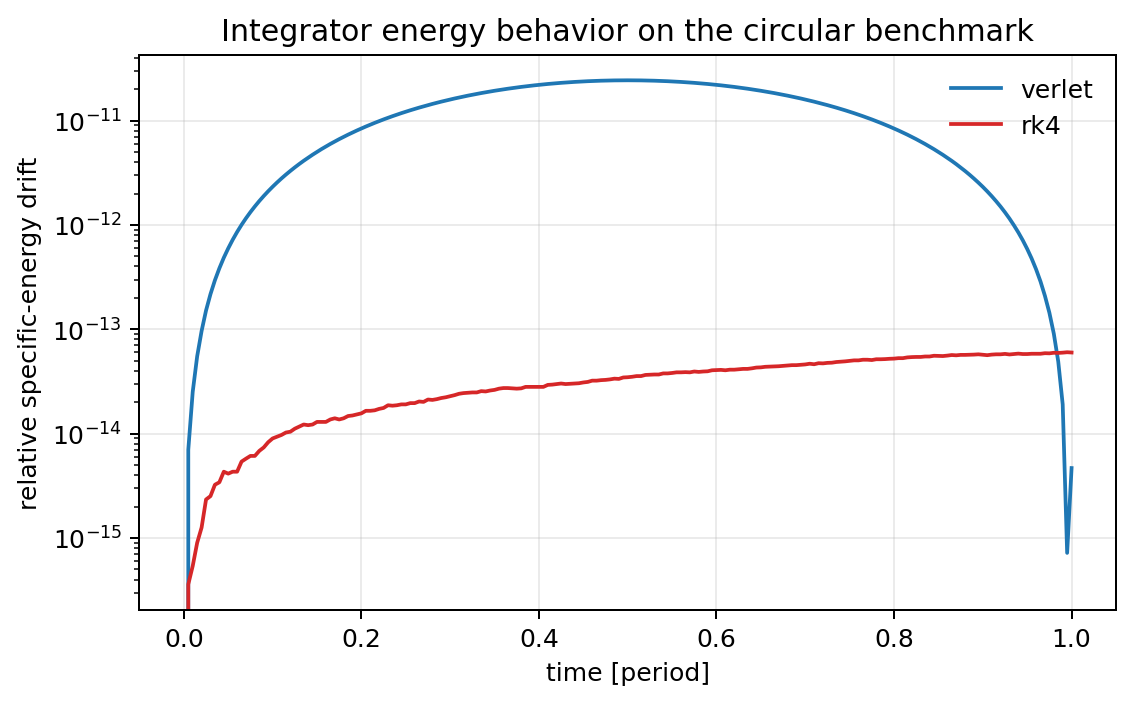
\includegraphics[width=\linewidth]{m8_energy_conservation.png}
\end{minipage}
\caption{M8：左为贴片圆锥绕日返回几何，右为圆轨道基准中的能量漂移。}
\label{fig:orbit-energy}
\end{figure}

\section{结论}

本项目已经完成 M1--M8 的必做内容。核心结论如下：
\begin{itemize}
    \item 贴片圆锥模型可以复现钱学森书中 $r_p=0.2\,\mathrm{AU}$ 的发射速度量级。
    \item 自建 N 体积分器在 M2 基准和 M3 历表对照中达到课程要求。
    \item 对深掠日返回轨道，单次月球借力确实能降低总 $\Delta v$，但由于来速很大，
    节省比例主要在 $1$--$2\%$ 量级。
    \item 2026 年最优发射窗口位于地球远日点附近；浅一些的掠日距离会显著降低总速度需求。
\end{itemize}

\section*{AI 使用说明}

本项目使用 Codex 协助环境搭建、模块接口设计、Python 数值脚本实现、Makefile 目标组织、
LaTeX 报告整理和运行结果核验。物理假设、课程要求解释、数值结果筛查与最终取舍均在本项目上下文中逐步完成。

\printbibliography

\end{document}
